\documentclass[11pt,a4paper]{article}

% ════════════════════════════════════════════════════════════════════
%  Federated Solar-Flare Prediction on SWAN-SF: A Provenance,
%  Leakage, and Evaluation-Protocol Audit  —  trimmed submission
%  edition. Structure follows the referee ship-list: provenance and
%  leakage, the leakage-free fold, persistence baselines, the two
%  BatchNorm findings, and calibration failure. The extended record
%  (experiment apparatus, LSTM/SMOTE/client studies, version
%  history) lives in the repository's full edition.
%  arXiv-preprint-style single-column manuscript
% ════════════════════════════════════════════════════════════════════

\usepackage{graphicx}
\usepackage{xcolor}
\usepackage{geometry}
\usepackage{amsmath}
\usepackage{amssymb}

\geometry{a4paper, top=2.6cm, bottom=2.6cm, left=2.5cm, right=2.5cm}

\usepackage{booktabs}
\usepackage{tabularx}
\usepackage{adjustbox}
\usepackage{enumitem}
\usepackage{caption}
\usepackage{microtype}
\usepackage{xurl}
\usepackage{placeins}

\captionsetup{font=small, labelfont=bf, skip=6pt}

\usepackage[numbers,sort&compress]{natbib}
\bibliographystyle{unsrtnat}

\usepackage[
    colorlinks=true,
    linkcolor=blue!55!black,
    citecolor=blue!45!black,
    urlcolor=blue!55!black,
    bookmarks=true,
    bookmarksnumbered=true,
    unicode=true,
    pdftitle={Federated Solar-Flare Prediction on SWAN-SF: A Provenance,
              Leakage, and Evaluation-Protocol Audit},
    pdfauthor={Deepanshu Balhara, Davesh Vats},
    pdfsubject={Federated Learning, Solar Flare Prediction, Benchmark
                Audit, Space Weather},
    pdfkeywords={federated learning, solar flare prediction, SWAN-SF,
                 benchmark audit, data provenance, evaluation protocol,
                 BatchNorm, non-IID data, class imbalance}
]{hyperref}

\widowpenalty=10000
\clubpenalty=10000
\emergencystretch=1.8em
\raggedbottom

\setlength{\parindent}{1.2em}
\setlength{\parskip}{2pt plus 1pt}

\newcommand{\R}{\mathbb{R}}
\newcommand{\E}{\mathbb{E}}
\newcommand{\w}{\mathbf{w}}
\newcommand{\norm}[1]{\left\lVert #1 \right\rVert}
\newcommand{\Fbeta}{F_{\beta}}

\title{Federated Solar-Flare Prediction on SWAN-SF: A Provenance,
Leakage, and Evaluation-Protocol Audit}
\author{Deepanshu Balhara \and Davesh Vats}
\date{October 2026}

\begin{document}

\thispagestyle{plain}

\begin{center}
    {\color{black!85}\rule{\textwidth}{0.4pt}}\\[2.2em]
    {\LARGE\bfseries Federated Solar-Flare Prediction on SWAN-SF:\\[0.35em]
     A Provenance, Leakage, and\\[0.15em]
     Evaluation-Protocol Audit\par}
    \vspace{1.6em}
    {\large Deepanshu Balhara\textsuperscript{1} \quad and \quad
     Davesh Vats\textsuperscript{2}\par}
    \vspace{0.7em}
    {\small\textit{Independent Researchers}\textsuperscript{1,2}\par}
    \vspace{1.1em}
    {\small October 2026\par}
    \vspace{1.4em}
    {\color{black!85}\rule{\textwidth}{0.4pt}}
\end{center}

\vspace{0.4em}

\begin{center}
\begin{minipage}{0.92\textwidth}
\footnotesize
\textbf{Abstract ---}
We audit federated learning on the public SWAN-SF solar-flare
benchmark. A provenance audit against the raw benchmark
(normalisation-invariant instance matching, 98.7--100\% coverage,
100\% test-side label agreement) shows that the cleaned export's
same-partition train/test pairing shares instances: every flaring
test window (6{,}234 of 6{,}234) also appears in training, and
85.7--90\% of training positives are synthetic. On a leakage-free,
temporally-preceding fold, discrimination generalises for every arm
(ROC-AUC 0.906--0.978) and the federated-versus-centralised gap
disappears; deployability is decided instead by persistence
baselines and calibration --- no arm beats same-region label
inertia (TSS 0.967), only XGBoost (0.848) and logistic regression
(0.489) clear 24-hour-lagged persistence (0.418), and no
validation-fit decision layer survives the $26\times$ prevalence
shift. Two apparent federated failures turn out to be BatchNorm
artefacts: the in-partition FedAvg collapse (0.575) is a composite
evaluation artefact, and on the raw, unbalanced substrate removing
BatchNorm alone restores the federated MLP (FedAvg 0.963/0.366,
FedProx 0.975/0.345, the latter matching the centralised MLP on
ROC-AUC within recorded retrain nondeterminism), while
pooled-statistics recalibration --- validated as an instrument on
the centralised model --- collapses every federated arm to chance,
a real finding. This is the first federated evaluation of SWAN-SF
and the first instance-level provenance audit of its cleaned
export. Every number regenerates from released result artefacts.

\vspace{0.55em}
\noindent\textbf{Keywords:} federated learning; solar flare
prediction; SWAN-SF; benchmark audit; data provenance; evaluation
protocol; BatchNorm; class imbalance

\vspace{0.55em}
\noindent\footnotesize Source code and all experimental artefacts:
\url{https://github.com/Daveshvats/Federated-Learning-for-Distributed-Space-Weather-Monitoring}
\end{minipage}
\end{center}

\vspace{0.8em}

\section{Introduction}\label{sec:intro}

Solar-flare prediction from photospheric magnetogram time series is a
benchmark-driven machine-learning problem. The community's public
reference is SWAN-SF~\cite{angryk2020}, and the literature on it has
grown around a small number of evaluation conventions: randomised
splits of pooled windows, a cleaned and rebalanced export, and a
reporting culture built on ROC/PR summary statistics. Those
conventions carry risk. The benchmark's own creators warned that
sliding-window temporal coherence ``invalidates the randomness
assumption, thus impacting all sampling
practices''~\cite{angryk2019}; subsequent work has echoed the
warning~\cite{ahmadzadeh2021}, and the cleaned export's release paper
explicitly prescribes pairing temporally-preceding training
partitions with a later test partition~\cite{eskandari2024}.
Flare-prediction models built on photospheric vector-magnetogram
summaries --- the SHARP parameter suite~\cite{bobra2015} --- have
demonstrated skilful classification of flaring versus non-flaring
active regions~\cite{leka2019,georgoulis2021}; the predictive signal
lives in quantities such as total unsigned current helicity,
magnetic free energy, and flux-emergence proxies.

Why federate a public benchmark whose data is freely poolable?
Methodologically, cross-silo federated
learning~\cite{mcmahan2017,kairouz2021} is the standard instrument
for studying non-IID data heterogeneity under a controlled protocol:
it prescribes exactly what moves between data holders (model
parameters) and exactly what does not (raw observations), which makes
it a clean lens for asking how much of a benchmark's apparent
difficulty survives when the data is deliberately fragmented.
Operationally, the SHARP-style parameters at the centre of this
pipeline are dominated by a single public instrument (SDO/HMI via
JSOC); the six-regional-agency narrative sometimes attached to
federated space-weather proposals does not describe this data and is
not claimed here. The six clients of this study are a simulation
protocol --- Dirichlet label skew across disjoint shards --- not a
claim about any institution. Federated flare forecasting itself is
not new (a federated transfer-learning preprint exists~\cite{fu2023});
what has not existed is a federated treatment of SWAN-SF that audits
its own benchmark artefacts before interpreting its numbers.

This paper provides that treatment, and its character is an audit.
We train six simulated clients on the benchmark in both its
cleaned/rebalanced and raw, naturally-imbalanced forms, under a
frozen evaluation protocol whose every selection decision is made on
validation data, and we ask three questions: what does a federated
pipeline actually achieve on SWAN-SF, what do the benchmark's own
artefacts do to the answer, and which parts of the observed behaviour
belong to the algorithms rather than to the evaluation machinery?
The contributions are:

\begin{enumerate}[leftmargin=2em, itemsep=3pt]
  \item \textbf{An instance-level provenance audit of the cleaned
  SWAN-SF export.} Normalisation-invariant matching against the raw
  benchmark (98.7--100\% coverage, 100\% test-side label agreement)
  shows the cleaned export's same-partition train/test pairing
  shares instances: every flaring test window (6{,}234 of 6{,}234) is
  in the training pool, and 85.7--90\% of training positives are
  synthetic (Section~\ref{sec:data}). The leakage phenomenon is
  documented prior art~\cite{angryk2019,eskandari2024}; the
  instance-level quantification inside a federated study is new.
  \item \textbf{A leakage-free federated evaluation.} On the
  temporally-preceding fold (train partitions 1--4, single-pass test
  on partition 5), all arms generalise (ROC-AUC 0.906--0.978) and the
  in-partition federated-versus-centralised gap disappears; event-level
  detection is essentially solved for every arm, and false-alarm
  burden --- not detection --- separates them
  (Section~\ref{sec:results}).
  \item \textbf{Corrected persistence baselines as the deployability
  verdict.} Same-region label inertia reaches TSS 0.967 with no
  learned model; only XGBoost (0.848) and logistic regression
  (0.489) clear 24-hour-lagged persistence (0.418) on TSS, and no arm
  clears it on HSS (Section~\ref{sec:results}).
  \item \textbf{Two BatchNorm findings that re-attribute apparent
  federated failures.} The in-partition FedAvg collapse (0.575) is a
  composite evaluation artefact --- untransported normalisation
  statistics compounded by a saturated validation monitor and the
  checkpoint rule it feeds; and on the raw, unbalanced substrate, an
  architecture-only control (three BatchNorm layers replaced by the
  identity, nothing else changed) restores the federated MLP to the
  centralised model's ROC-AUC level, so the collapse is dominated by
  BatchNorm under federation, not by the flattened-feature encoder
  and not by federation per se (Section~\ref{sec:results}).
  \item \textbf{A calibration failure that is real, not an
  artefact.} Pooled-statistics recalibration --- validated as an
  instrument on the centralised model, where it reproduces the
  model's own statistics to within $7\times10^{-5}$ ROC-AUC ---
  collapses every federated arm to chance on the raw substrate, so a
  pooled-statistics transport fix would not rescue federation there;
  and no validation-fit decision layer survives the $26\times$
  prevalence shift between the balanced training partitions and the
  natural-prevalence test (Section~\ref{sec:calibration}).
  \item \textbf{A frozen, reproducible protocol.} Immutable splits,
  validation-only selection and calibration, single-pass test
  evaluation, and machine-readable artefacts for every number
  reported here, released with the code.
\end{enumerate}

We make no operational alerting claim. The benchmark's data is
public and freely poolable; the downstream
flare$\to$CME$\to$storm$\to$GIC chain is physically far from the
quantity modelled and is not evaluated (see~\cite{boteler2019} for
that literature).

\section{Related work}\label{sec:related}

Three literatures meet in this study. First, flare prediction from
magnetogram summaries: the SHARP parameter
suite~\cite{bobra2015} established the feature vocabulary; benchmark
comparisons~\cite{leka2019,georgoulis2021} established the
verification culture (TSS, HSS, reliability, persistence baselines)
that Section~\ref{sec:results} applies; and the FLARECAST
programme~\cite{georgoulis2021} established the operational framing.
SWAN-SF itself~\cite{angryk2020} contributed the partitioned
benchmark with multivariate time-series windows, and its cleaned
release~\cite{eskandari2024} contributed the rebalanced export whose
provenance Section~\ref{sec:data} audits. The benchmark's creators
have been explicit about the sampling hazard since
2019~\cite{angryk2019}, and the cleaned release prescribes
temporally-preceding folds --- warnings this paper quantifies at the
instance level and then obeys.

Second, federated learning. FedAvg~\cite{mcmahan2017} and
FedProx~\cite{li2020} are the workhorse algorithms evaluated here;
the cross-silo survey of Kairouz et
al.~\cite{kairouz2021} frames the methodology. The known interaction
between federation and normalisation layers is the FedBN line of
work~\cite{li2021fedbn}: BatchNorm running statistics do not
transport with parameters, and the interaction can masquerade as a
federated optimisation failure. Section~\ref{sec:results} shows two
instances of exactly that masquerade on this benchmark, one of them
compounded by a saturated drift monitor. Class imbalance under
federation connects to focal loss~\cite{lin2017} and its federated
adaptations~\cite{sarkar2020}, and to oversampling
approaches~\cite{chawla2002} whose value on this benchmark the
extended record quantifies as a clean negative at natural
prevalence.

Third, federated space weather. Federated flare forecasting exists
as a 2023 transfer-learning preprint~\cite{fu2023}; the present
study is, to the authors' knowledge, the first federated evaluation
of SWAN-SF, the first instance-level provenance audit of its cleaned
export, and the first leakage-free re-evaluation of federated flare
prediction under the benchmark's intended protocol. Federated
learning has proven transformative in settings where privacy
constraints really are binding~\cite{rieke2020}; no such constraint
is claimed for this public data, and the federation here is a
controlled heterogeneity instrument rather than a privacy solution.

\section{The benchmark, its cleaned export, and the leakage
audit}\label{sec:data}

\paragraph{SWAN-SF and the two substrates.}
SWAN-SF~\cite{angryk2020} partitions solar-active-region time series
into five folds of 60-minute, $60\times24$ multivariate windows over
24 SHARP-style magnetic-flux parameters, with a binary M/X-class
flare label on every window. The community mostly consumes its
\emph{cleaned} export~\cite{eskandari2024}: under-sampled negatives,
Tomek-cleaned boundaries, TimeGAN-augmented positives, imputed
values, and per-partition normalisation --- a pre-balanced substrate
(48.9\% training prevalence) whose natural-prevalence test
partitions carry 1.31--1.88\% positives. This study evaluates on
both substrates: the cleaned export as shipped, and a raw substrate
rebuilt in-pipeline from the raw benchmark (the release's imputation
and normalisation reproduced from their published description, every
parameter fitted on training data only, verified against the
released export on the audit-matched windows, series differences
bounded by $5\times10^{-3}$ at float16 storage). The raw substrate
removes the synthetic positives and the $26\times$ prevalence shift
and asks the classical question: can the models learn the natural
distribution at all?

\paragraph{The provenance audit.}
The cleaned export carries no region or event identifiers, so the
audit first aligns every cleaned window to its raw instance. The raw
benchmark (Harvard Dataverse) encodes, per instance, the flare
class, the HARP region identifier, and window timestamps in its
filenames. The matching key is the per-feature argmax/argmin
position along the 60 timesteps --- 48 discrete invariants that
survive any per-feature monotone normalisation and are robust to the
export's imputation noise. A window is accepted as aligned when at
least 28 of 48 invariants agree (borderline cases additionally
require mean per-feature Spearman $\rho \ge 0.70$). On the test
partitions this verifies 98.7--100.0\% of windows with 100.00\% label
agreement; on the training side, label agreement is 99.71\% (161
disagreements, which bound the synthetic-share estimate below).

\paragraph{What the audit found.}
Three structural facts follow. First, the test export of partition
$p$ contains \emph{all} raw instances of $p$; the counts match
exactly on every partition. Second, the training export of $p$ is a
rebalanced \emph{subset of the same instances}: the verified training
pool covers 56{,}005 unique raw instances, every one of which is
also a test instance (56{,}005/56{,}005) --- and every M/X-flaring
test instance (6{,}234 of 6{,}234, 100\% of the minority class) is
in the training pool. Third, 85.7--90.0\% of the training positive
windows are TimeGAN-synthetic (they have no raw counterpart), while
virtually no negative windows are. The release paper prescribes
pairing temporally-preceding training partitions with a later test
partition; a pipeline that instead pools the training exports and
evaluates on the same partitions' test exports --- the default
drift of any naive consumer --- partially measures memorised data,
most severely for the minority class. Because no HARP region spans
two partitions (verified: 0 shared HARPs), a temporally-preceding
fold is automatically instance-, region-, and time-disjoint.

\paragraph{The leakage-free fold.}
All headline comparisons are therefore re-run under the benchmark's
intended protocol: training on the training exports of partitions
1--4 (77{,}865 windows; 65{,}406 train / 12{,}459 validation after a
stratified carve), and a single-pass evaluation on the test export
of partition 5 (75{,}365 windows, natural 1.31\% prevalence). The raw
substrate uses the same partition structure, so its fold is
leakage-free by the same construction. Everything else is frozen:
six Dirichlet-sketched clients, 50 rounds, seed 42, the focal loss
and calibration machinery of Section~\ref{sec:method}.
Figure~\ref{fig:partition} shows the client partition the federated
arms actually train on.

\begin{figure}[t]
\centering
\begin{adjustbox}{max width=0.88\textwidth}
    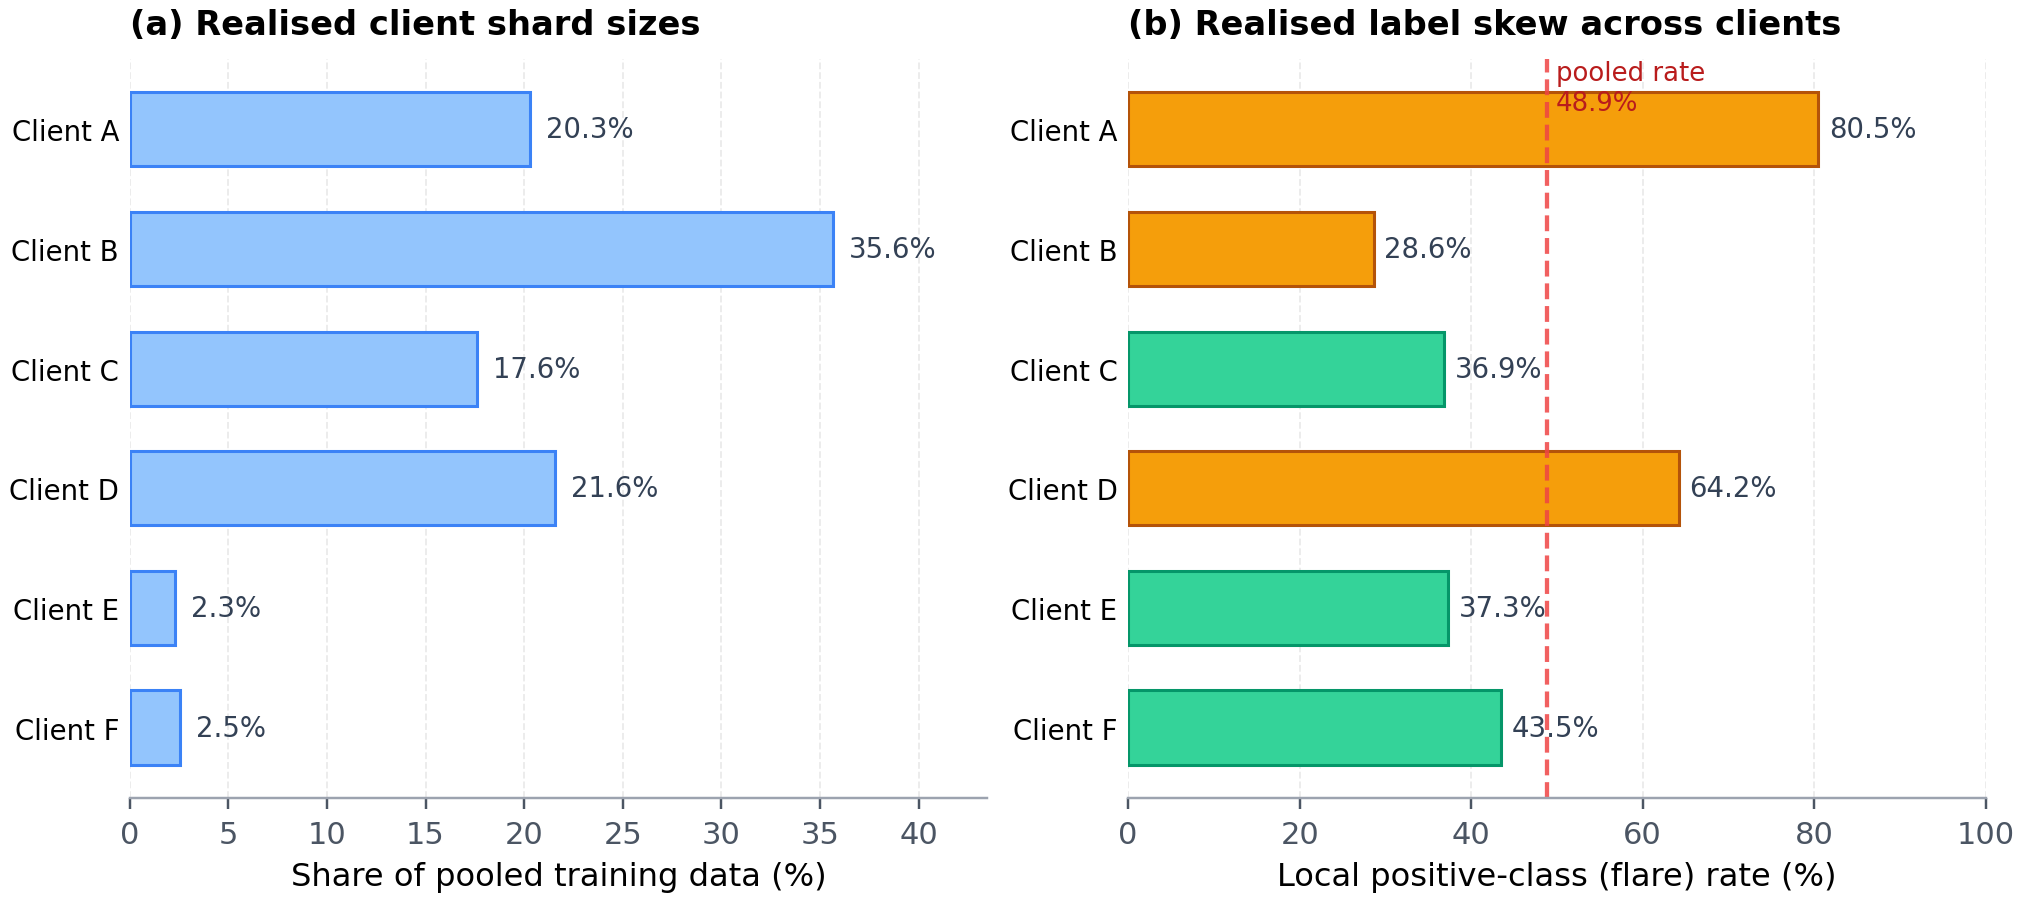
\includegraphics{figures/fig_partition.png}
\end{adjustbox}
\caption{Non-IID partitioning of the pooled training data into six
simulated clients by label-aware Dirichlet sampling (concentration
$\alpha = 1.0$, seed 42). Proportions are read directly from the
frozen run's cached client assignment: the shard sizes and label
skews are the heterogeneity every federated arm of this paper
trains under.}
\label{fig:partition}
\end{figure}

\section{Federated protocol}\label{sec:method}

\paragraph{Simulated cross-silo federation.}
Six simulated clients (neutral labels A--F; no institution
participates) hold disjoint shards of the training pool, partitioned
by a Dirichlet($\alpha{=}1.0$) label-skew draw. Each round, a random
subset of clients trains the shared architecture locally; the server
averages the returned \emph{parameters} (size-weighted FedAvg
\cite{mcmahan2017}); FedProx \cite{li2020} adds the proximal term
($\mu = 0.01$) to the local objective. Raw observations never move
--- the transport contract that makes the heterogeneity study
controlled. The local objective is a server-aware federated focal
loss \cite{lin2017,sarkar2020} with the focusing parameter clamped
for stability under extreme imbalance.

\paragraph{Architectures.}
The MLP arm consumes the standard flattened feature encoding of the
$60\times24$ window (six summary statistics per magnetic parameter;
144 features) through a three-layer network with BatchNorm and
dropout (29{,}377 parameters). The architecture control of
Section~\ref{sec:results} replaces the three \texttt{BatchNorm1d}
layers with the identity and changes nothing else (28{,}929
parameters) --- no running statistics exist, so parameter transport
is exact. A sequence arm (SolarLSTM, 219{,}265 parameters, consuming
the raw $60\times24$ series directly, no BatchNorm) provides the
BatchNorm-free architecture comparator; its full study lives in the
extended record. Centralised references (logistic regression,
XGBoost, the pooled MLP and LSTM of identical architecture) are
trained on the pooled data under the same budget conventions.

\paragraph{Frozen evaluation contract.}
Splits are immutable. Threshold and calibration selection happen on
validation only; test evaluation is single-pass. Operating points
are reported two ways: at the validation-selected $F_2$-optimal
threshold, and at validation-frozen fixed-FPR targets (0.5/1/2/5\%),
which are invariant to monotone miscalibration and to prevalence.
Neural posteriors pass a prior-shift calibrator fit on validation
before thresholding. Checkpoint selection is the best-validation-$F_1$
rule, with the selected round and a validation-ROC-selected
sensitivity row disclosed beside it and per-round test trajectories
recorded as diagnostics; no test-based selection happens anywhere.
Verification metrics (TSS, HSS, Brier skill, 10-bin reliability,
climatology) accompany every stored operating point, and persistence
baselines are computed on the true time order within each active
region, as the verification culture mandates.

\paragraph{Reproducibility.}
Every number in this paper regenerates from machine-readable result
artefacts committed with the code; the underlying dataset cache is
frozen under a 20-file SHA-256 manifest verified by a released
script, and an independent re-execution from the public artefacts
reproduces the in-partition headline metrics exactly. The extended
record in the repository carries the full apparatus: five-seed
statistics, the component-ablation grid, client-level holdouts, the
sequence-arm and oversampling studies, and the audit trail of every
protocol defect found and fixed along the way.

\section{Results}\label{sec:results}

\subsection{The leakage-free fold: discrimination survives, the
federation gap does not}

Table~\ref{tab:leakfree} compares the five headline arms on the
leakage-free fold against the shipped in-partition numbers. Three
observations follow. First, \emph{discrimination generalises}: every
arm attains at least 0.906 ROC-AUC on the unseen partition, and the
task is easier than the in-partition protocol suggested (logistic
regression reaches 0.978/0.455). Second, the
centralised-versus-federated gap of the in-partition protocol
\emph{disappears}: the pooled MLP of identical architecture reaches
0.973/0.382 against FedProx's 0.976/0.308 --- a 0.003 ROC difference
and a reversed PR ordering. The in-partition gap (0.888 vs 0.954) was
an artefact of the protocol pairing, not a federation effect. Third,
the FedProx-versus-FedAvg contrast only partially survives: FedProx
leads by 0.070 ROC-AUC but trails FedAvg by 0.062 PR-AUC, and the
next subsection shows why neither difference should be read as an
algorithm property while BatchNorm sits in the loop.

\begin{table}[t]
\centering
\caption{Leakage-free fold (train partitions 1--4, single-pass test
on partition 5, natural 1.31\% prevalence) against the shipped
in-partition numbers. Threshold-conditional calibration metrics use
the validation-frozen prior-shift pipeline; ROC/PR are
threshold-free.}
\label{tab:leakfree}
\small
\begin{tabular}{@{}l c c c c c c c@{}}
\toprule
 & \multicolumn{2}{c}{\textbf{In-partition}} &
 \multicolumn{5}{c}{\textbf{Leakage-free fold}} \\
\cmidrule(r){2-3} \cmidrule(l){4-8}
\textbf{Model} & ROC & PR & ROC & PR & Brier & ECE & R@2\%FPR \\
\midrule
Logistic regression & 0.824 & 0.235 & 0.978 & 0.455 & 0.375 & 0.477 & 0.695 \\
XGBoost (centralised) & 0.977 & 0.493 & 0.971 & 0.457 & 0.055 & 0.101 & 0.692 \\
Centralised MLP & 0.888 & 0.153 & 0.973 & 0.382 & 0.544 & 0.687 & 0.555 \\
FedAvg MLP & 0.575 & 0.199 & 0.906 & 0.370 & 0.127 & 0.337 & 0.652 \\
FedProx MLP & 0.954 & 0.307 & 0.976 & 0.308 & 0.271 & 0.508 & 0.631 \\
\bottomrule
\end{tabular}
\end{table}

The calibration and threshold-transfer failures persist
leakage-free --- the balanced-validation carve (48.9\% prevalence)
again faces the natural-prevalence test (1.31\%), the same 26-fold
prior shift without the instance overlap --- so they are genuine
properties of the balanced-training/natural-test interface rather
than overlap artefacts: the validation-frozen FPR operating points
are violated by every arm (XGBoost realises 15.3\% FPR at the frozen
2\% target; FedProx 49.4\%), and only XGBoost's posteriors remain
usable (Brier 0.055 versus 0.127--0.544 for the neural arms).

\paragraph{Persistence baselines set the deployability floor.}
The toolkit of Leka et al.~\cite{leka2019} --- TSS, HSS,
persistence, climatology --- accompanies every operating point, and
the persistence baselines set two floors that are not decorative.
Same-region previous-window persistence (label inertia) achieves
TSS 0.967 / HSS 0.970 on the partition-5 test with no learned model
at all: at a 24-hour label horizon on $\sim$60-minute windows, an
active region that is flaring is still flaring, and \emph{no arm in
this paper --- XGBoost included --- beats that floor}. The
24-hour-lagged variant (forecast = the label of the same-region
window nearest $t-24$\,h) scores TSS 0.418 / HSS 0.434; on TSS,
XGBoost (0.848) and logistic regression (0.489) are the only arms
above it, and every neural arm at its frozen threshold sits below
it, while on HSS no arm clears the floor at all (XGBoost's HSS is
0.201). This is the classic Leka-era result, and a benchmark audit
is the right vehicle for stating it plainly: at this window geometry
the honest question is not whether models beat persistence, but
whether anything beats \emph{lagged} persistence --- and on this
fold, at TSS, two arms do, none at HSS. A committed sensitivity sweep
over eight candidate lag definitions agrees: the seven point-lag
variants land at TSS 0.392--0.418 with the same two arms clearing
each, while a lookback-flare variant scores 0.964 --- label inertia
under another name, which no arm clears.

\paragraph{Event-level evaluation.}
Regrouping the partition-5 test decisions into physical flare events
(65 true M/X-class events, validation-frozen thresholds, 1-hour
alert cooldown; Table~\ref{tab:eventlevel}), all five arms detect
effectively every event (64--65 of 65) with a median first-alert
lead of 23.4\,h before flare peak. That lead must be read for what it
is: the label is positive for every window in the 24 hours before a
flare, so a median first alert near the horizon's edge measures the
label boundary, not precursor physics. What separates the arms is
their false-alarm burden: XGBoost emits 1.7 false-alarm windows per
day versus 11.6--12.7 for the neural arms --- a $7\times$ difference
that mirrors the window-level calibration gap and confirms that the
deployability boundary on this benchmark is calibration, not
detection.

\begin{table}[t]
\centering
\caption{Event-level metrics on the leakage-free fold (65 true
M/X-class events, validation-frozen $F_2$ thresholds, 1-hour alert
cooldown). FA = false alarm.}
\label{tab:eventlevel}
\small
\begin{tabular}{@{}l c c c c@{}}
\toprule
\textbf{Model} & \textbf{Events detected} & \textbf{FA windows/day} &
\textbf{Alerts/day} & \textbf{Lead to peak (h)} \\
\midrule
Logistic regression & 65/65 (100\%) & 8.6 & 8.8 & 23.4 \\
XGBoost (centralised) & 64/65 (98.5\%) & 1.7 & 1.9 & 23.3 \\
Centralised MLP & 65/65 (100\%) & 12.7 & 12.8 & 23.4 \\
FedAvg MLP & 65/65 (100\%) & 11.6 & 11.8 & 23.4 \\
FedProx MLP & 65/65 (100\%) & 11.9 & 12.1 & 23.4 \\
\bottomrule
\end{tabular}
\end{table}

\subsection{The raw substrate: an apparent federated collapse}
\label{sec:rawcollapse}

Retraining the identical frozen protocol on the raw, unbalanced
benchmark separates the arms decisively (Table~\ref{tab:rawsubstr}).
The centralised arms are substrate-robust (logistic regression
unchanged to the third decimal; the centralised MLP's PR-AUC
\emph{rises} from 0.382 to 0.445; XGBoost's falls from 0.457 to
0.329 --- the synthetic positives were inflating its minority-class
precision, not teaching it). The federated MLP arms are not: FedAvg
falls to 0.875/0.056 with its calibrated posteriors never crossing
the validation-frozen threshold (test recall 0.000), FedProx to
0.930/0.149, and FedAvg detects \emph{zero} of the 65 events. Read
naively, this is a federation failure. The next two subsections show
it is mostly a BatchNorm artefact.

\begin{table}[t]
\centering
\caption{Raw-substrate retraining (train raw partitions 1--4,
natural 2.05\% prevalence, imputation and normalisation reproduced
in-pipeline with train-only parameters; single-pass test on raw
partition 5, natural 1.31\% prevalence; identical frozen protocol).
The leakage-free cleaned-substrate fold is reproduced for
comparison.}
\label{tab:rawsubstr}
\small
\begin{tabular}{@{}l c c c c c c@{}}
\toprule
 & \multicolumn{2}{c}{\textbf{Fold (cleaned)}} &
 \multicolumn{4}{c}{\textbf{Raw substrate}} \\
\cmidrule(r){2-3} \cmidrule(l){4-7}
\textbf{Model} & ROC & PR & ROC & PR & Brier & R@2\%FPR \\
\midrule
Logistic regression & 0.978 & 0.455 & 0.978 & 0.448 & 0.053 & 0.732 \\
XGBoost (centralised) & 0.971 & 0.457 & 0.974 & 0.329 & 0.018 & 0.587 \\
Centralised MLP & 0.973 & 0.382 & 0.971 & 0.445 & 0.010 & 0.596 \\
FedAvg MLP & 0.906 & 0.370 & 0.875 & 0.056 & 0.013 & 0.063 \\
FedProx MLP & 0.976 & 0.308 & 0.930 & 0.149 & 0.032 & 0.343 \\
\bottomrule
\end{tabular}
\end{table}

\subsection{BatchNorm finding 1: the in-partition collapse is a
composite evaluation artefact}

The client MLPs contain three \texttt{BatchNorm1d} layers, and local
training updates their running statistics every batch --- but the
federation transports \emph{parameters only}: running statistics are
buffers, not parameters, and buffers never move. The server-side
global model therefore evaluates with its initialisation buffers
forever (the shipped checkpoints carry \texttt{num\_batches\_tracked}
$=0$, \texttt{running\_mean} $=0$, \texttt{running\_var} $=1$ after
50 rounds), where each BN layer degenerates to the fixed affine map
$x\gamma+\beta$. The second half of the mechanism is the saturated
monitor: with init buffers, evaluated probabilities squeeze into a
narrow band, validation $F_1$ pins to its all-positive closed form
$2p/(1+p)$, and the best-validation checkpoint rule --- acting on
that saturated signal --- restored the round-20 FedAvg state over the
healthy round-5 state.

Table~\ref{tab:bndiag} decomposes the published in-partition FedAvg
numbers: the frozen 50-round protocol was re-run faithfully and the
identical global weights evaluated at three rounds under four BN
treatments. The verdict is unambiguous. The weights never lost
discriminative content: under evaluation-time batch statistics the
round-50 state --- whose shipped evaluation is 0.098, below chance
--- holds 0.953 ROC-AUC, and the round-20 state the rule shipped
holds 0.951. The in-partition collapse to 0.575 is a composite
evaluation artefact: untransported normalisation statistics ---
a mechanism documented since FedBN~\cite{li2021fedbn} and analysed
in subsequent BatchNorm-under-federation
studies~\cite{wang2023bn,guerraoui2024bn,bnscaffold2024} ---
compounded by a saturated monitor and the checkpoint rule it feeds.
A controlled
no-BN re-training in-partition confirms the training-side reading:
with the three BN layers removed and nothing else changed, neither
FedAvg nor FedProx diverges, the validation monitor stays
informative, and the 0.379 ROC-AUC gap between the two shipped
artefacts shrinks to 0.002--0.036 at every round.

\begin{table}[t]
\centering
\caption{Test ROC-AUC / PR-AUC of the identical in-partition FedAvg
global weights under four BatchNorm treatments (frozen protocol,
seed 42). Round 20 is the state the shipped checkpoint rule
returned. Arm D is what a buffer-transporting implementation would
have evaluated.}
\label{tab:bndiag}
\small
\begin{tabular}{@{}l c c c@{}}
\toprule
\textbf{BN treatment} & \textbf{Round 5} & \textbf{Round 20} & \textbf{Round 50} \\
\midrule
A: init buffers (shipped) & 0.950 / 0.264 & 0.575 / 0.199 & 0.098 / 0.010 \\
B: recalibrated (pooled) & 0.786 / 0.044 & 0.893 / 0.099 & 0.881 / 0.086 \\
C: batch statistics & 0.946 / 0.328 & 0.951 / 0.329 & 0.953 / 0.288 \\
D: transported round buffers & 0.885 / 0.157 & 0.931 / 0.194 & 0.935 / 0.209 \\
\bottomrule
\end{tabular}
\end{table}

\subsection{BatchNorm finding 2: removing BatchNorm restores the
federated MLP on the raw substrate}

The decisive control applies the same intervention to the raw
substrate: retrain both federated MLP arms with the three
\texttt{BatchNorm1d} layers replaced by the identity, changing
nothing else (same frozen protocol, shards, budget, aggregation,
seed). Table~\ref{tab:rawnobn} reports the outcome. FedAvg gains
$+0.088$ ROC-AUC and $+0.310$ PR-AUC ($6.5\times$); FedProx gains
$+0.045$ and $+0.196$. In gap terms: FedAvg's ROC gap to the
centralised MLP closes from 0.096 to 0.008 (91\%) and its PR gap
from 0.389 to 0.079 (80\%); FedProx's ROC gap closes \emph{past}
zero ($-0.004$ residual) and its PR gap from 0.296 to 0.100 (66\%).
Both no-BN arms sit level with their BatchNorm-free sequence
counterparts on ROC-AUC (FedAvg 0.963 vs the sequence arm's 0.958;
FedProx 0.975 vs 0.970), and no-BN FedProx \emph{matches} the
centralised MLP on ROC-AUC (0.975 vs 0.971): the $-0.004$ residual
sits inside the retrain nondeterminism the replication record
documents for exactly these arms (gate deltas $-0.002$ to $+0.023$
ROC-AUC), so the single-seed reading is parity within noise, not
federated precedence. The raw-substrate collapse of the BN-carrying
MLP arms is therefore dominated by BatchNorm under federation ---
not by the flattened-feature encoder, and not by federation per se.
Two boundaries keep the claim honest: (a) PR-AUC, not ROC-AUC, is
where work remains (no-BN FedProx's 0.345 sits below the centralised
MLP's 0.445 and the sequence arm's 0.404) --- what these arms
license is the attribution, not a new state-of-the-art row; (b) the
level claims now carry a second seed: re-executed at seed 43
(initialisation and shard draw reseeded, validation carve
unchanged), the shipped selections move by at most 0.002 ROC-AUC
(FedAvg 0.963$\to$0.961, FedProx 0.975$\to$0.976) and at most
0.024 PR-AUC without overturning an ordering, while the thresholded
validation-$F_1$ monitor is the seed-sensitive layer (best values
0.53$\to$0.66 and 0.09$\to$0.30) --- at 2\% prevalence the rank
metrics, not the monitor, carry the conclusions
(Section~\ref{sec:discussion}).

\begin{table}[t]
\centering
\caption{No-BatchNorm control on the raw substrate (single
intervention: three \texttt{BatchNorm1d} layers $\to$ identity,
nothing else changed; reference rows read from the released
artefacts).}
\label{tab:rawnobn}
\small
\begin{tabular}{@{}l c c@{}}
\toprule
\textbf{Arm (raw substrate)} & \textbf{ROC-AUC} & \textbf{PR-AUC} \\
\midrule
FedAvg MLP (BatchNorm, published) & 0.875 & 0.056 \\
FedAvg MLP (no BatchNorm, this control) & 0.963 & 0.366 \\
FedProx MLP (BatchNorm, published) & 0.930 & 0.149 \\
FedProx MLP (no BatchNorm, this control) & 0.975 & 0.345 \\
\midrule
Centralised MLP (reference) & 0.971 & 0.445 \\
FedAvg LSTM (reference, no BatchNorm) & 0.958 & 0.305 \\
FedProx LSTM (reference, no BatchNorm) & 0.970 & 0.404 \\
\bottomrule
\end{tabular}
\end{table}

\paragraph{The validation divergence, honestly.}
FedAvg's no-BN test ROC-AUC \emph{declines} from 0.974 (round 5) to
0.963 (round 50) while its validation ROC-AUC and $F_1$ still
improve (0.974 to 0.977; 0.345 to 0.527), so the shipped
best-validation rule selects the weakest test-ROC round of its own
monitored trajectory. A prevalence difference cannot explain this
divergence: ROC-AUC is a rank statistic, invariant to class
prevalence, so the validation carve's 2.05\% against the test fold's
1.31\% moves thresholded quantities, not the ranking. Two candidate
mechanisms remain, both testable with the released region-disjoint
split generator: the random validation carve shares active regions
with the training shards (the same leakage class the provenance
audit documents benchmark-wide), and partition 5 is the temporally
latest fold, so late-round specialisation to partitions 1--4 can
register as validation gain and test loss at once. The
within-fold region-disjoint validation re-run of both arms is
prepared in the released code and is the first remaining compute
item; FedProx's trajectory, for contrast, climbs monotonically from
0.931 to 0.975 --- the proximal term's stabilisation becoming
visible precisely once BatchNorm is removed.

\section{Calibration: the deployability boundary}\label{sec:calibration}

\paragraph{The prior shift is first-class.}
The validation prevalence (48.9\%) and the test prevalence
(1.9--1.31\%) differ by a factor of 26 because the cleaned benchmark
ships pre-balanced training partitions and natural-prevalence test
partitions. The frozen protocol forbids using test labels ---
including test prevalence --- for any selection, so the prior-shift
calibrator is fit with the validation prevalence as its deployment
target. The consequence is quantitative: at the frozen thresholds,
FedProx's calibrated Brier (0.264) and ECE (0.496) are \emph{worse
than the climatology's} (0.239, 0.470), i.e.\ at natural prevalence
the neural posterior is not deployment-usable as a probability,
while the XGBoost reference suffers the least (Brier 0.063, ECE
0.115). Rebalanced training data invalidates naive threshold
transfer: an $F_2$-optimal threshold at 49\% prevalence is
semantically meaningless at 1.9\%. The correct deployment
instrument, pending full recalibration, is the recall-at-fixed-FPR
operating point, which is invariant to monotone miscalibration and
to prevalence.

\paragraph{The calibration-arm comparison is a clean negative.}
Five calibration arms (raw, prior-shift, Platt, isotonic,
temperature), each fit on the balanced validation set and applied
once to the test set, with the arm selected by minimum validation
Brier --- a proper scoring rule, so the selection itself is honest.
The outcome: minimum validation Brier selects isotonic for all three
neural models (validation Brier 0.012--0.025), and the selection is
\emph{wrong} --- the selected arms' test Brier (0.352--0.541) is the
worst of the five, because the balanced validation set rewards
aggressive recalibration that the natural-prevalence test then
punishes. No validation-fit decision layer survives the shift.

\paragraph{Pooled recalibration collapses federation: a real
finding.}
Could a statistics-transport fix rescue the BatchNorm-carrying
federated arms? The BN diagnostic's pooled arm (B) --- exact
per-client statistics pooled by the law of total variance --- is the
oracle for exactly that fix, and on the raw substrate it
\emph{collapses} the federated arms to chance (0.500--0.501), even
though in-partition the same oracle \emph{recovered} FedAvg from
0.575 to 0.893. The instrument itself is validated: applied to the
centralised raw MLP, where it should reconstruct the model's own
statistics, it reproduces the ROC-AUC to within $6.8\times10^{-5}$
(0.96864 vs 0.96870). So the collapse is a real finding, not a bug:
pooling exact per-client normalisation statistics across six
heterogeneous raw-prevalence clients inflates variance past the
point where any single pooled normalisation ranks the test
distribution. A pooled-statistics transport fix would not rescue
federation on the raw substrate --- removing the BN layers (or
transporting per-client buffers) is the class of fix that works,
and the no-BN control of Section~\ref{sec:results} is its direct
proof.

\paragraph{What survives, end to end.}
Ranking survives everywhere for the centralised arms and, once
BatchNorm is removed, for the federated arms. Probabilities survive
only for XGBoost. Thresholds frozen at balanced prevalence transfer
for nothing. Same-region label inertia remains unbeaten at TSS.
The deployability boundary is calibration, and on this benchmark it
is drawn by the prevalence shift the cleaned export itself
introduced.

\section{Discussion and limitations}\label{sec:discussion}

\paragraph{What this audit changes.}
For benchmark consumers, the instance-level audit turns a documented
warning~\cite{angryk2019,eskandari2024} into a measured quantity:
same-partition pairing on the cleaned export puts 100\% of the
minority test class into training, so in-partition numbers on that
pairing partially measure memorisation. The leakage-free fold --- the
benchmark's own intended protocol --- is the honest instrument, and
on it the apparent federated-versus-centralised gap vanishes. For
federated-learning practitioners, the two BatchNorm findings are the
lesson: normalisation layers whose statistics do not transport can
manufacture both a catastrophic collapse and a stabilisation
narrative (FedProx's apparent safety was, in large part, compatibility
with the untransported evaluation path), and a saturated validation
monitor converts an evaluation defect into a checkpoint-selection
defect. The engineering conclusion is BatchNorm plus buffer
transport, or BatchNorm-free architectures --- not BN removal as a
general remedy, since the BN architecture is genuinely useful under
correct normalisation.

\paragraph{Limitations and remaining work.}
The honest caveats, each with the instrument that would upgrade the
claim: the leakage-free fold is a single fold and seed (fold
replication breadth is prepared in the released runners); the no-BN
control's level claims --- sequence-arm parity and
centralised-MLP parity --- sit inside the recorded retrain noise
band, a boundary its second-seed replication confirms (both arms
within 0.002 ROC-AUC of their seed-42 selections); the random
validation carve
inside the raw-substrate protocol may share active regions with the
training shards, and the region-disjoint re-run that separates that
hypothesis from temporal drift is likewise prepared in the released
code (roughly 1.7\,kiloseconds of GPU compute for both arms); the
event-level results are single-fold with Wilson half-widths of
$\pm$2.8--4.0 detection points; the calibration analysis shows no
validation-fit decision layer survives the prior shift, but
prior correction toward an \emph{estimated} deployment prevalence
from unlabelled data remains unstudied; and the SCAFFOLD
implementation measured in the extended record departs from the
reference algorithm in disclosed ways (a sign-inverted
control-variate update among them), so its cells there are
implementation-case evidence and no conclusion of this paper rests
on them. Cryptographic privacy, poisoning defence, and the
downstream GIC chain are out of scope.

\paragraph{Conclusion.}
Federated solar-flare prediction on SWAN-SF, evaluated honestly, is
neither a failure nor a win: it is a mirror for the evaluation
protocol. On the leakage-free fold every arm generalises and
federation costs nothing measurable; on the raw substrate the
apparent federated collapse is BatchNorm's, not federation's, and
removing the layers restores parity with the centralised model; the
real failures are inherited from the benchmark --- a prevalence
shift that no validation-fit decision layer survives, and a
persistence floor that no learned model beats at this label
geometry. The audit instruments themselves --- instance-level
provenance matching, the BN-transport diagnostic, the
instrument-validated pooled-recalibration oracle --- are released
and reusable, and they are the contribution most likely to outlive
this benchmark.


\FloatBarrier
\bibliography{refs}

\end{document}
